\documentclass[12pt]{article}

\usepackage{float}
\usepackage{amsmath}    % need for subequations
\usepackage{graphicx}   % need for figures
\usepackage{verbatim}   % useful for program listings
\usepackage{color}      % use if color is used in text
\usepackage{subfigure}  % use for side-by-side figures
\usepackage{hyperref}   % use for hypertext links, including those to external documents and URLs
\usepackage[utf8]{inputenc}
\usepackage[T1]{fontenc}

\hypersetup{
    colorlinks=true,
    linkcolor=blue,
    urlcolor=red,
    linktoc=all
}
% don't need the following. simply use defaults
\setlength{\baselineskip}{16.0pt}    % 16 pt usual spacing between lines

\setlength{\parskip}{3pt plus 2pt}
\setlength{\parindent}{20pt}
\setlength{\oddsidemargin}{1cm}
\setlength{\evensidemargin}{1cm}
\setlength{\marginparsep}{0.75cm}
\setlength{\marginparwidth}{2.5cm}
\setlength{\marginparpush}{1.0cm}
\setlength{\textwidth}{150mm}

\begin{comment}
\pagestyle{empty} % use if page numbers not wanted
\end{comment}

\renewcommand{\contentsname}{Table des matières}

\begin{document}

\begin{center}
{\large \textbf{Documentation de la Classe Math} \\ % \\ = new line
Projet GL groupe 17 \\
22 janvier 2018
\end{center}

\newpage
\tableofcontents
\newpage


\section{Introduction}
Afin de rendre le language Déca plus complet dans le cadre d'une utilisation scientifique, nous avons
décidé d'implémenter la bibliothèque standard Math. Celle-ci contient les fonctions trigonométriques
élémentaires tel que \textbf{cosinus}, \textbf{sinus}, \textbf{arctangent}, \textbf{arcsinus} et \textbf{arccosinus}.
A celles-ci s'ajoute la fonction \textbf{ulp}, qui est une fonction indispensable pour les calculs flottants.
Enfin, pour des raisons pratiques, il a été choisi d'enrichir cette classe des fonctions usuelles comme
\textbf{pow}, \textbf{fact} et \textbf{sqrt}. \\
L'implémentation de ces fonctions requiert une bonne sensibilité aux calculs flottants et aux erreurs
entrainées. En effet, en plus des erreurs mathématiques, il faut prendre en compte les erreurs informatiques
pour obtenir des résultats correctes pour un grand ensemble d'arguments. C'est là que se trouve toute la
subtilité et la difficulté du développement d'une telle classe. Pour l'ensemble des fonctions, et de manière plus générale,
 pour le language Deca, nous utilisons les flottants IEEE754 simple précision (encodé sur 32 bits). \\
Bien que nous sommes conscient que les fonctions présentées ici ont déjà été implémentées et de manière
plus précise dans la plupart des languages, nous sommes convaincus qu'être averti des erreurs machines
et des solutions possibles sont des compétences incontournables pour un ingénieur en informatique.


\section{Rappel sur les flottants IEEE754 simple précision}

\subsection{Notions générales}
\label{sec:notions}

La représentation des flottants simple précision en machine se fait sur 32 bits.\\
-1 bit pour le signe \\
-8 bits pour l'exposant \\
-23 bits pour la mantisse/significant/precision (+1 bit implicite) \\

\begin{figure}[!h]
    \begin{center}
      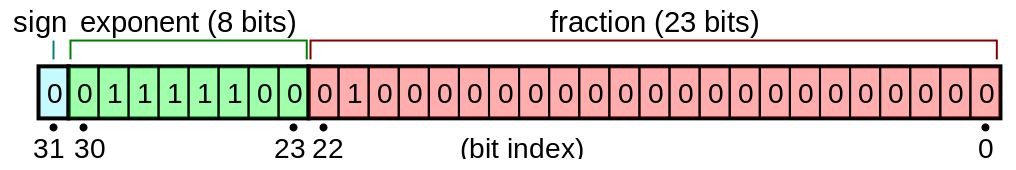
\includegraphics[scale=0.35]{32-float.png}
      \caption{Nombres flottants simple précision.}
      \label{Représentation en machine des nombres flottants simple précision.}
    \end{center}

\end{figure}

La valeur du flottant est ensuite calculée par la formule suivante:
\begin{center}
\begin{equation}
       val =  (-1)^{b_{31}} * (1.b_{22}b_{21}...b_0)_2 * 2^{(b_{30}b_{29}...b_{23})_2 - 127}
\end{equation}
\end{center}

L'exposant détermine entre quelle puissance de deux le flottant se situe. En simple précision nous pouvons
énumérer des flottants positif entre $[2^{e_{min}}, 2^{e_{max}}[ =  [2^{-149}, 2^{127}[$. On remarque également
avec la formule que lorsque l'exposant est fixé, nous pouvons toujours énumérer le même nombre de flottant, celui-ci
étant de $2^{precision - 1}$. \\
Les intervalles de puissance de 2 n'étant pas constant mais ayant toujours un
nombre de flottant constant à l'intérieur nous amène à la conclusion que l'espace entre les flottants n'est pas
constante, mais dépendante de l'exposant du flottant. \\
Il a y plus de flottant autour des petites valeurs et moins autour des grandes valeurs.\\

\begin{figure}[!h]
    \begin{center}
      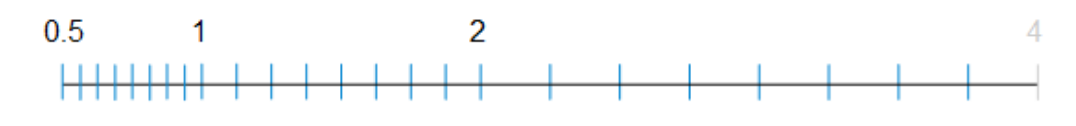
\includegraphics[scale=0.35]{repartition-float.png}
      \caption{Répartition des flottants (4 bits de précision)}
      \label{Exemple de répartition de flottants avec 4 bits de précision}
    \end{center}
\end{figure}

Cette partie est essentielle pour comprendre les problèmes que l'ont essaye de
résoudre dans ce travail.
L'enjeux de cette extension est donc d'évaluer des fonctions mathématiques usuelles avec le maximum de précision
possible tout en gérant la contrainte d'un environnement fini et discret.

\subsection{Les modes d'arrondi}
\label{sec:arrondis}
Lorsque l'on rentre un flottant à la main, ou bien que le résultat d'un calcul entre flottant n'abouti pas à
un nombre machine (quasiment tout le temps), comment le processeur attribut-il un flottant représentable en machine?\\
\\
C'est là qu'intervient le \textbf{mode d'arrondi} du compilateur. Il nous permet de passer de l'ensemble
des valeurs continues à l'ensemble discret représentable en machine. Il existe plusieurs modes d'arrondi,
 les plus utilisés
sont Round to Nearest (RN), Round Down (RD), Round Up (RU) ou encore Round Zero (RZ).\\
A chaque fois que la valeur d'une variable x n'est pas représentable en machine, la fonction d'arrondi
transforme x tel que:\\

\begin{center}
  $round(x) = x(1 + \delta)$  avec $|\delta| < 2^{-(p-1)}$ et $p$ la précision
\end{center}

avec $|\delta| < 2^{-p}$ dans le cas où le mode d'arrondi est RN. C'est le mode que nous utilisons
pour toute cette classe car il permet de réduire l'erreur moyenne par rapport aux autres modes.\\
Cette partie est également indispensable car c'est ici que l'on comprends d'où vient l'erreur informatique
qui va s'ajouter à l'erreur mathématique dans l'approximation de nos fonctions.


\section{Utilisation pratique}

Cette partie donne les détails d'utilisation des fonctions implémentées ainsi que les valeurs de
retour attendue.
\begin{itemize}

\item \textbf{float ulp(float x);}

Comme expliqué dans la \hyperref[sec:notions]{partie 2.1}, l'espace entre deux flottants successifs n'est pas constant.
Cette méthode renvoie la distance du flottant en argument avec le prochain flottant supérieur représentable.
Pour les valeurs extrême, nous avons $ulp(0) = 2^{-149}$ et $ulp(2^{127}) = 2^{104}$. Cette fonction
nous sera très utile pour évaluer nos algorithmes.

\item \textbf{float sin(float x)/cos(float x);}

Accepte n'importe quel flottant en argument.\\
Renvoie le flottant le plus proche possible (moins d'un ulp si possible) du sinus/cosinus de l'angle x en radian.
Les valeurs de retours sont dans l'intervalle $[-1,1]$.

\item \textbf{float atan(float x);}

Accepte n'importe quel flottant en argument.\\
Renvoie le flottant le plus proche possible (moins d'un ulp si possible) de l'arctangente de x.
Les valeurs de retours sont dans l'intervalle $[-\frac{\pi}{2}, \frac{\pi}{2}]$.

\item \textbf{float asin(float x);}

N'accepte que des arguments dans l'intervalle $[-1,1]$.\\
Renvoie le flottant le plus proche possible (moins d'un ulp si possible) du sinus/cosinus de l'angle x en radian.
Les valeurs de retours sont dans l'intervalle $[-\frac{\pi}{2}, \frac{\pi}{2}]$.
Nottons que $asin(-1) = -\frac{\pi}{2}$ et $asin(1) = \frac{\pi}{2}$.

\item \textbf{float acos(float x);}

N'accepte que des arguments dans l'intervalle $[-1,1]$.\\
Renvoie le flottant le plus proche possible (moins d'un ulp si possible) du sinus/cosinus de l'angle x en radian.
Les valeurs de retours sont dans l'intervalle $[0, \pi]$. \\
Nottons que $acos(-1) = \pi$ et $asin(1) = 0$.

\item \textbf{float pow(float x, int n);}

Pas de restriction sur les arguments. Renvoie le flottant $x$ élevé à la puissance n. \\
Nottons que $pow(x, 0) = 1$ peut importe $x$.

\item \textbf{int fact(int n);}

N'accepte que des entiers n positifs. Renvoie le produit $n*(n-1)*...*1$. \\
Nottons que $fact(0) = 1$.

\item \textbf{float sqrt(float x);}

Cette fonction n'accepte que des flottants positifs.
Elle renvoie le flottant $f$ le plus proche possible tel que $f*f = x$. \\
Nottons que $sqrt(0) = 0$ et $sqrt(1) = 1$.

\end{itemize}


\section{Choix des algorithmes}
\subsection{Cosinus et sinus}
\subsubsection{Range reduction: Cody and Waite}
\label{sec:rangered}

La première étape pour évaluer les fonctions sinus et cosinus consiste à se ramener à un intervalle réduit tel
que $[0, \pi]$, $[0, \frac{\pi}{2}]$ ou encore $[0, \frac{\pi}{4}]$ pour ensuite reconstruire les fonctions
en utilisant leurs propriétés de périodicité, de parité et quelques formules trigonométriques.\\
\\
Un simple modulo pourrait fonctionner, mais il a un impacte terrible sur la précision. \\
En effet le nombre $\frac{\pi}{4}$ n'est pas représentable en machine. Ainsi lorsque l'on fait un modulo
$\frac{\pi}{4}$, à chaque fois que nous enlèvons/ajoutons $\frac{\pi}{4}$ à notre argument, nous introduisons
l'erreur correspondante à la distance entre $\frac{\pi}{4}$ et sa représentation en machine à laquelle s'ajoute
l'arrondi du résultat (RN) de l'addition/soustraction.\\
Le modulo réalisé s'écrit alors mathématiquement:
\begin{center}
\begin{equation}
  x = RN(x - RN(k\frac{\pi}{4})))}
\end{equation}
\end{center}
avec $k = (int) \frac{x}{\frac{\pi}{4}}$


Ainsi lorsque l'entier k est grand (ie quand l'argument de la fonction est grand) l'erreur
introduite devient trop importante. Les algorithmes de range réduction cherchent à résoudre ce problème.
\\
\\
Nous avons appliqué la méthode de Cody and Waite au 4ème degré. Cette méthode a l'avantage d'être simple
à comprendre et d'offrir de bon résultat. Cependant elle n'est pas suffisante pour les très grandes valeurs
(plus de $10^6$).\\
Cette méthode consiste à séparer la variable C ($C = \frac{\pi}{4}$ dans notre cas) en plusieurs autres variables
tel que:\\
$C = C1 + C2$, \\
$C1 \simeq \frac{\pi}{4}$  est un nombre machine le plus proche possible de C, \\
$C2 = \frac{\pi}{4} - C1$ est appelé le résidu (non représentable en machine). \\
\\
Ainsi le modulo se transforme en:
\begin{center}
\begin{equation}
$$x = RN((x - RN(kC1)) - RN(kC2)) = RN((x - kC1) - RN(kC2))$$
\end{equation}
\end{center}

En effet C1 étant un nombre machine, nous pouvons réaliser sa soustraction exactement
sans erreur. La méthode de Cody and Waite au degré 4 étend seulement cette notion
à 4 constantes C1, C2, C3 et C4, pour gagner en précision.\\
\\
Dans notre cas nous avons donc pour $C = \frac{\pi}{4}$:\\

\noindent C1 = 0.78515625  //representable en machine \\
C2 = 0.00024187564849853515624  //représentable en machine \\
C3 = 0.000000037747668102383613583  //représentable en machine\\
C4 = 0.00000000000128167207614641725  //reste\\


On peut trouver plus d'information sur cette méthode en page 5 de Ref.~\cite{paper1}.\\
Maintenant que nous sommes sur notre intervalle réduit $[0, \frac{\pi}{4}]$, il nous faut
approximer nos fonctions. Il existe une méthode appelée CORDIC qui ne demande
que très peu de calcul pour un resultat correct. Cette technique était employée
dans les anciennes calculettes qui n'avaient pas beaucoup de puissance de calcul.\\

Mais au vu du manque de précision de ses resultats, nous avons décidez
d'utiliser d'autres méthodes afin d'approcher les fonctions de manière polynômiale. \\
Nous avons implémenter deux techniques différentes à savoir la décomposition en
série de Maclaurin et l'approximation par polynôme minimax.

\subsubsection{Serie de Maclaurin}
Les séries de Maclaurin sont une généralisation des séries de Taylor lorsque
l'on ne part pas de la valeur 0 de la variable.\\
Voici l'expression de cette série pour le sinus:
\begin{center}
\begin{equation}
 sin(x) = \sum_{n=0}^{\infty} \frac{(-1)^n}{(2n+1)!}x^{2n+1}
\end{equation}
\end{center}
et pour le cosinus:
\begin{center}
\begin{equation}
  cos(x) = \sum_{n=0}^{\infty} \frac{(-1)^n}{(2n)!}x^{2n}
\end{equation}
\end{center}

En prenant les 8 premiers termes pour le cosinus par exemple nous obtenons un polynôme
que l'on réécrit sous la forme de \textbf{polynôme de Horner}. Nous obtenons
le résultat suivant:

\begin{center}
\begin{equation}
  cos(x) \simeq 1 + x^2(c_1 + x^2(c_2 + x^2(c_3 + x^2(c_4 + x^2(c_5 + x^2(c_6 + x^2(c_7 +x^2c_8)))))))
\end{equation}
\end{center}
avec $c_i = \frac{1}{(2i)!}$.\\
\\
Cette forme représente deux gros avantages du point de vu de la précision. \\
\\
-Tout d'abord, contrairement à l'écriture suggérée par la somme (6), on commence ici par sommer ensemble
les petites valeurs $(c_7 +x^2c_8)$ ce qui permet de réduire ce qu'on appelle l'erreur
d'absorption. \\
Un exemple d'erreur d'absorption est la somme $10^7 + 10^{-7}$ qui donne en machine
un résultat de $10^7$. \\
\\
-Le deuxième point forme de cette écriture est la mise en évidence d'opérations de forme
$(ab + c)$ car cela va nous permettre d'utiliser l'\textbf{instruction FMA} (Fused Multiply Addition)
qui réalise cette opération disponible sur la plupart des processeurs récents.\\
Chaque opération en machine a un coût en terme d'erreur et de temps, l'instruction FMA
nous permet d'introduire une seule erreur lors de son appel contre deux pour le classique
$(ab + b)$. En effet, elle renvoie le flottant représentable le plus proche du produit $(ab + c)$.\\
D'un point de vu mathématique, si a, b et c sont des nombres machines on a:

\begin{center}
\begin{equation}
  |fma(a,b,c) - (ab+c)| \leq \frac{1}{2}ulp(ab+c)
\end{equation}
\end{center}

Elle rend également l'exécution plus rapide. Pour plus d'informations sur FMA
se rendre à Ref.~\cite{paper2}.\\
\\
De cette manière, nous pouvons approcher nos fonctions sur l'intervalle réduit puis les reconstruire
pour obtenir l'ensemble de définition complet. Cependant une autre approche qui se veut
plus précise a été implémenté: le polynôme Minimax.

\subsubsection{Polynôme Minimax}
\label{sec:minimax}

Le polynôme Minimax est une alternative aux séries de Maclaurin pour évaluer une fonction
une fois que l'ensemble de définition a été réduit.\\
\\
L'idée du polynôme Minimax part du théorème mathématique de Weierstrass qui dit que toute
fonction continue peut être approchée autant que l'on veut par un polynôme:\\
\\
\textbf{Théorème Weierstrass:} \textit{Soit f une fonction continue sur [a, b], pour tout
$\epsilon > 0$ il existe un polynôme p tel que $||f-p||_{\infty} \leq \epsilon$.}\\
\\
avec $$||f-p||_{\infty} = \max_{a \leq x \leq b}|f(x)-p(x)|$$.\\
\\
Ainsi le polynôme Minimax est le polynôme $p^*$ tel que:
\begin{center}
\begin{equation}
  ||f-p^*||_{\intfy} = \min_{p \in P_n}||f-p||_{\infty} = \min_{p \in P_n}(\max_{a \leq x \leq b}|f(x)-p(x)|)
\end{equation}
\end{center}
D'où le nom de polynôme Minimax. Pour des explications plus approfondies sur ces polynômes,
se referer à Ref.~\cite{elementaryFunctions} page 32.\\
En informatique nous imposons en plus de cela des contraintes sur les coefficients de $p^*$.
Par exemple, nous voulons que ceux-ci soient représentables parfaitement en machine et \lt 1.\\
Déterminer ces coefficients est un problème difficile, il existe pour cela différents outils,
tel que Sollya Tool ou Mapple. Ces logiciels prennent en argument la fonction à approximer, les bornes, la précision
désirée et le degré du polynôme voulu. Ils renvoient, si possible, les coefficients représentables en machine
du polynôme minimax. Pour plus d'information sur ces outils, rendez-vous sur Ref.~\cite{sollya}.\\

Une fois les coefficients déterminés, nous utilisons une fois de plus la \textbf{forme de Horner}
et l'\textbf{instruction FMA} pour conserver un maximum de précision dans les calculs.

\subsection{Arctangent, arcsinus et arccosinus}
Comme nous pouvons déduire la fonction arcsinus et arccosinus de la fonction arctangente par la formule
de trigonométrie $asin(x) = atan(\frac{x}{\sqrt{1-x^2}})$ et $acos(x) = \frac{\pi}{2} - asin(x)$, nous
nous intéressons principalement à cette dernière.

\subsubsection{Séparation de l'ensemble de définition}
De la même manière que pour les fonctions sinus et cosinus, la première étape de l'approximation
consiste à trouver un intervalle de définition réduit qui nous permettra par la suite de
reconstruire la totalité de la fonction.\\
\\
Dans le cas de l'arctangente, nous utilisons la propriété suivante:\\
\begin{center}
  $atan(x) + atan(1/x) = sign(x)\frac{\pi}{2}$ pour $x \in R^*$.
\end{center}
Ce qui nous permet de réduire l'intervalle à $[-1, 1]$, en prenant l'inverse de l'argument $x$ si
$|x| > 1$.

\subsubsection{Polynôme minimax}

Nous utilisons ici aussi un polynôme Minimax, basé sur les mêmes principes que ceux
expliqués en \hyperref[sec:minimax]{partie 4.1.3}. Avec l'outil Sollya, nous obtenons un polynôme
de degré 17 $P = x+x^3(C1 + x^2(C2+x^2(C3+x^2(C4+x^2(C5+x^2(C6+x^2(C7+C8x^2)))))))$
dont les coefficients machines sont:\\

\noindent C8 = 0x1.6d2026p-9f\\
C7 = -0x1.03f2d4p-6f\\
C6 = 0x1.5beeb4p-5f\\
C5 = -0x1.33194ep-4f\\
C4 = 0x1.b403a8p-4f\\
C3 = -0x1.22f5c2p-3f\\
C2 = 0x1.997748p-3f\\
C1 = 0x1.5554d8p-2f\\
\\
Ce polynôme approxime ici la fonction arctangente sur $[-1, 1]$.\\
\\

Une fois de plus nous tirons profit de la forme de Horner pour le polynôme obtenu ainsi que
de l'instruction FMA du compilateur, afin de conserver un maximum de précision vis-à-vis du
résultat. L'implémentation complète se trouve dans le code de la fonction.


\subsection{Unit in the Last Place (ULP)}
La fonction ULP doit déterminer la distance entre le flottant en argument et le suivant. Comme
expliqué en \hyperref[sec:notions]{partie 2.1}, il suffit de déterminer entre quelles puissances de 2
notre argument se trouve. Ou encore, de retrouver la valeur de l'exposant dans la représentation
du flottant dans la machine.\\
\\
L'algorithme pour déterminer la valeur de l'exposant est assez simple, en partant de
exposant =0, il suffit de:\\
- Si l'argument est inférieur à 1, alors nous le multiplions par deux jusqu'à obtenir une valeur
entre $[1, 2]$ tout en soustrayant 1 à l'exposant à chaque multiplication.\\
- Si l'argument est supérieur à 1, alors nous le divisons par deux jusqu'à obtenir une valeur
entre $[1, 2]$ tout en additionnant 1 à l'exposant à chaque division.\\
\\
Nous avons choisi de manière arbitraire l'intervalle $[1, 2]$ comme point de référence car il correspond
à l'intervalle $[2^e, 2^{e+1}]$ pour un exposant nul. Un autre intervalle peut tout à fait
fonctionner du moment que l'on soustrait bien l'exposant de référence au resultat obtenu.\\
\\
Une fois que nous avons la valeur de l'exposant, l'ULP correspondant est égal à
la largeur de l'intervalle $[2^e, 2^{e+1}]$ divisé par le nombre de flottant dans l'intervalle
c'est-à-dire $2^{precision - 1}$.\\
On arrive alors a la formule suivante:

\begin{center}
\begin{equation}
  ulp(x) = 2^{e + 1 - p}
\end{equation}
\end{center}
avec e l'exposant de $x$ et $p$ la précision du système flottant en question (ici $p=24$).\\




\section{Analyse théorique de la précision des algorithmes}
\subsection{Précision de l'algorithme de Range Reduction}

Nous étudions l'erreur engendrée par l'algorithme \textbf{reduction3} qui implémente
une réduction de Cody and Waite au quatrième degré dont le principe est expliqué en
\hyperref[sec:rangered]{partie 4.1.1}.\\
\\
Voici une comparaison des erreurs de l'algorithme de range réduction et
de l'algorithme naif du modulo. Nous prenons ici comme point de repère le modulo
en double précision de java.lang.Math.PI.

\begin{figure}[ht]
    \begin{center}
      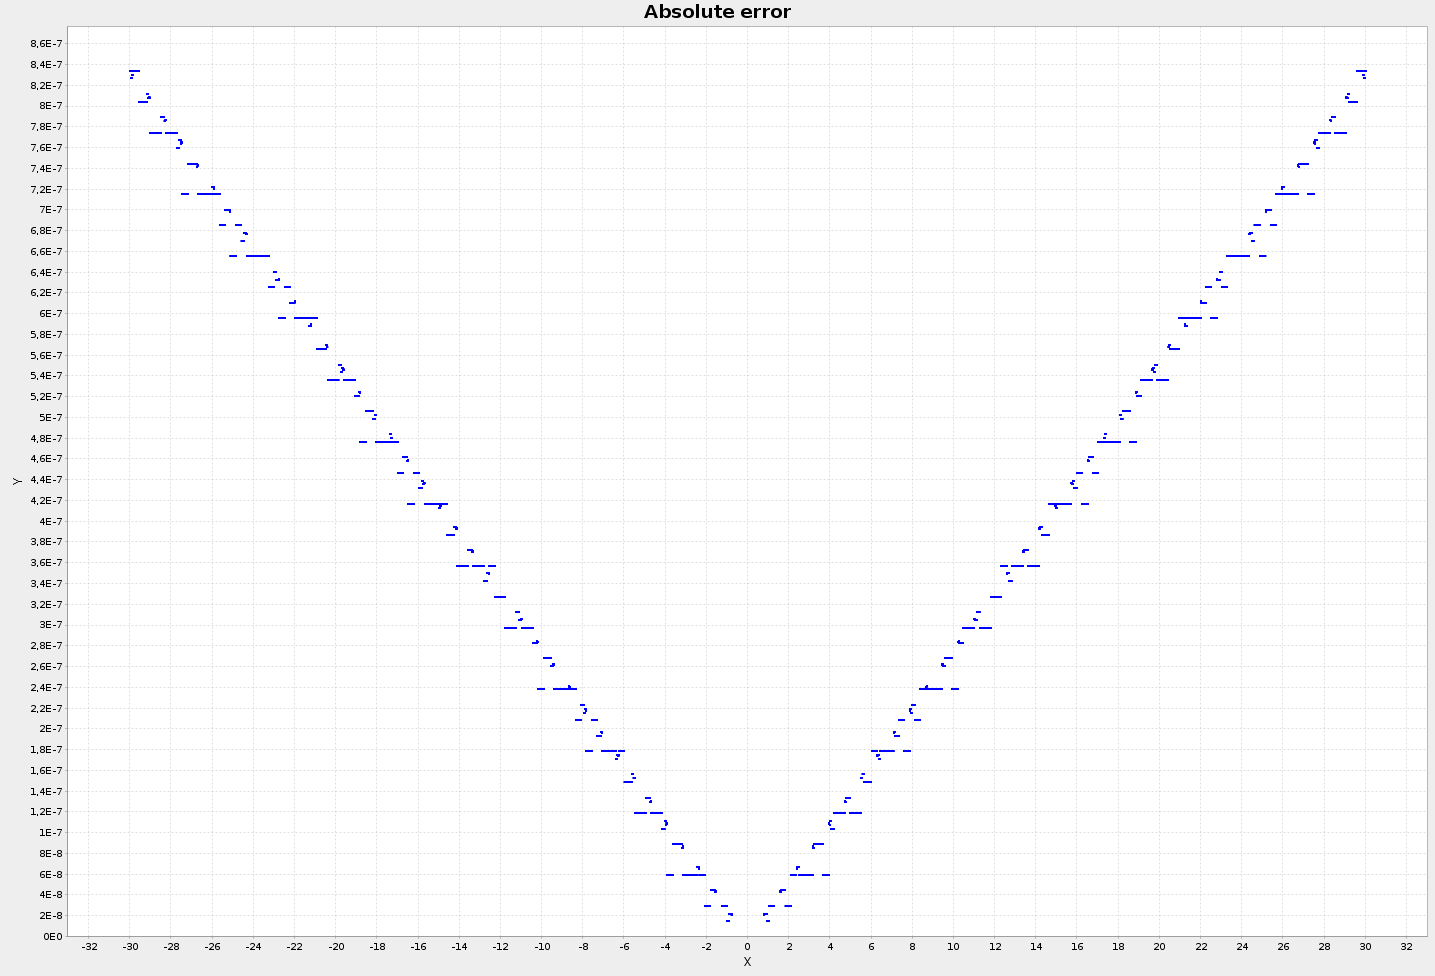
\includegraphics[scale=0.28]{AbsoluteErrorNoRangeRed.png}
      \caption{Erreur absolue de reduction avec modulo naif dans [-30,30]}
      \label{Erreur absolue de reduction avec modulo naif}
    \end{center}
\end{figure}

\begin{figure}[ht]
    \begin{center}
      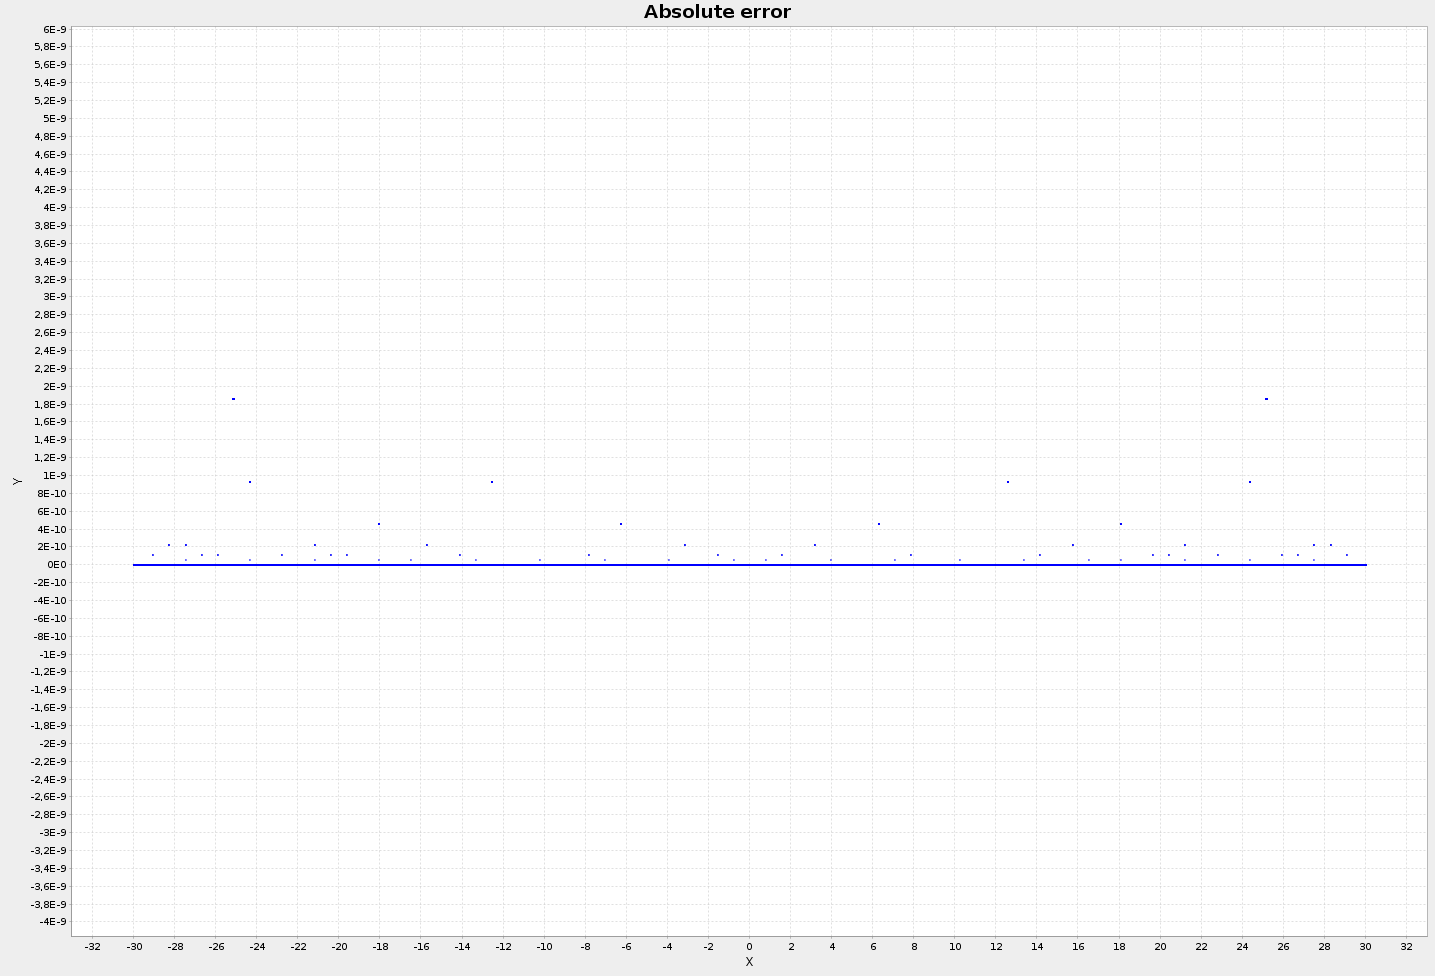
\includegraphics[scale=0.28]{AbsoluteErrorRangeRed.png}
      \caption{Erreur absolue de reduction avec Cody and Waite dans [-30,30]}
      \label{Erreur absolue de reduction avec Cody and Waite}
    \end{center}
\end{figure}
\\
\\
Dans la première figure nous voyons que le modulo introduit une erreur qui évolue de manière
linéaire par rapport à k. En effet, $\frac{\pi}{4}$ contient 8 digits décimaux de précision en flottant
de simple précision. Ainsi
nous introduisons une erreur en $O(10^{-8})$ à chaque soustraction/addition de $\frac{\pi}{4}$.\\
\\
L'algorithme de Cody and Waite correspond lui à l'opération suivante:
\begin{center}
\begin{equation}
  RN((((x - kC1) - kC2) - kC3) - RN(kC4))
\end{equation}
\end{center}
avec $k = (int) x / \frac{\pi}{4}$.\\ \\
Ici l'opération $(((x - kC1) - kC2) - kC3)$ se réalise sans erreur car C1, C2 et C3 sont des flottants machine.
Ainsi comme \\ \\
C4 = 0.00000000000128167207614641725 (= 1.28167207614641725E-12) \\ \\
nous gagnons 12 digits décimaux de précision sur la réduction de l'argument. Ceci n'est pas négligeable comme le montre les graphiques.
\\ \\

La linéarité de l'erreur par rapport à $k$ suffit pour justifier que nos algorithmes sinus et cosinus
ne sont plus valable pour de grands argument ($> 10^6$) à cause de la range reduction.
Non seulement parce que l'erreur commise est trop
importante, mais aussi parce que un nouveau phénomène apparait.

\begin{figure}[ht]
    \begin{center}
      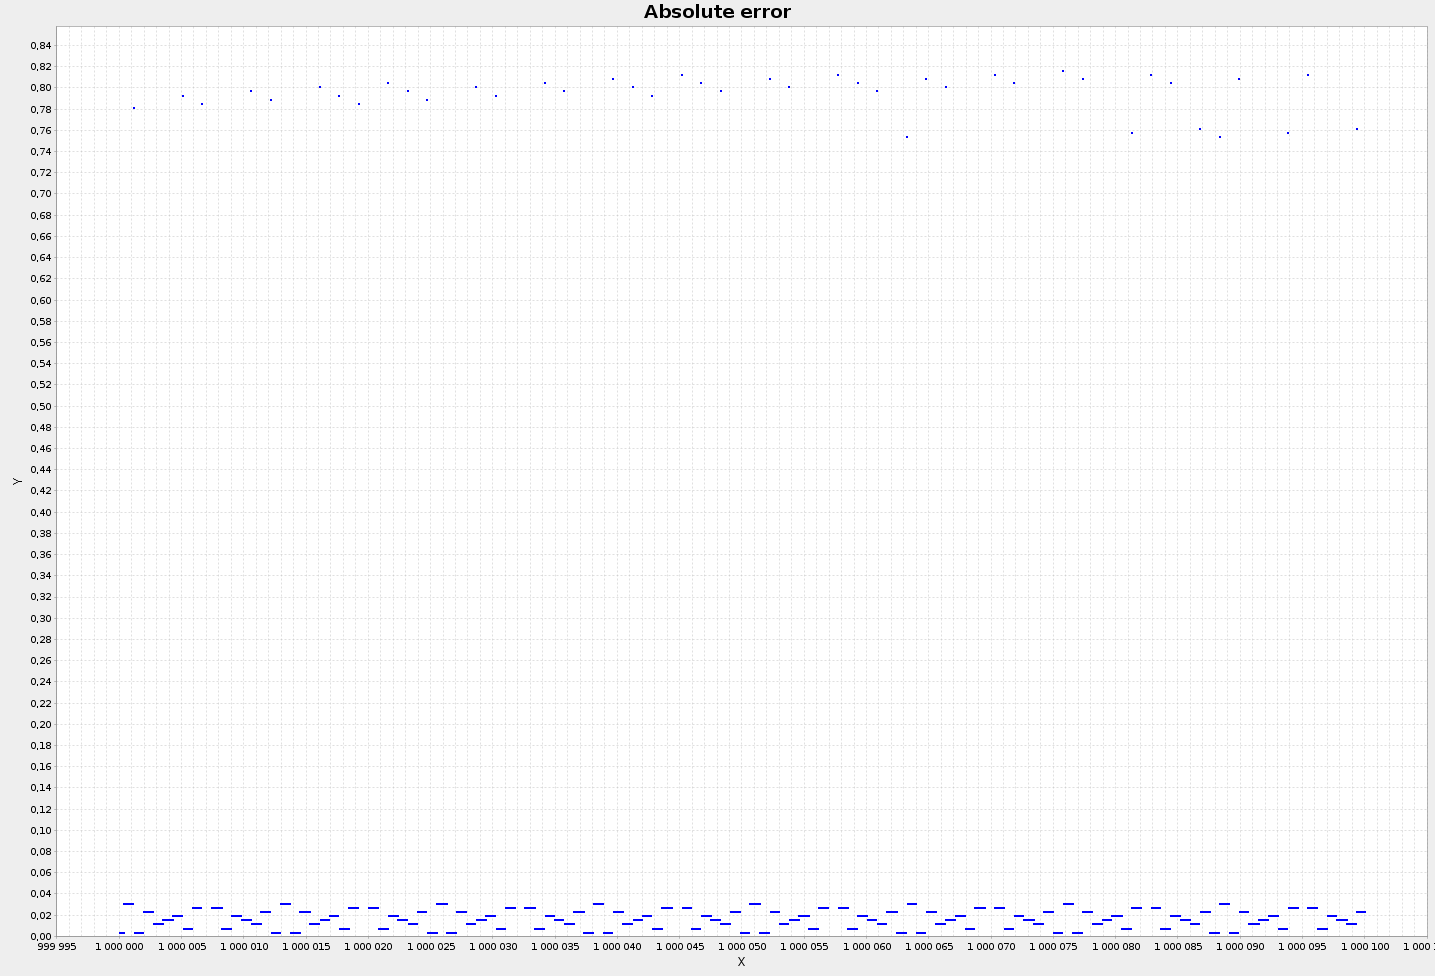
\includegraphics[scale=0.28]{AbsoluteErrorRangeRedFar.png}
      \caption{Erreur absolue de reduction avec Cody and Waite dans [10^6,10^6 + 100]}
      \label{Erreur absolue de reduction avec Cody and Waite}
    \end{center}
\end{figure}

On voit clairement que pour les grands arguments la précision est mauvaise (erreur en $10^{-2}$). On
observe en plus de cela des erreurs absolues très grande, de l'ordre de $\frac{\pi}{4}$. \\
Cela vient du faite que la valeur entière $k$ a été faussée lors de son calcul ($k = (int) x / \frac{\pi}{4}$)
à cause de la
représentation en machine de $\frac{\pi}{4}$.\\
Dans la littérature, on appelle cela "Worste case for Range Reduction".\\
Ce phénomène ne se produit qu'a partir du moment où la valeur du 7ème digit de $\frac{\pi}{4}$ a un impacte
dans le calcul de k ($(int) x / \frac{\pi}{4}$) c'est-à-dire quand $x \geq 10^6$.
\\
\\
Pour pallier au problème des très grands arguments, il faut considérer un second algorithme de range réduction
appelé \textbf{algorithme de Payne-Hanek}. Celui-ci n'a cependant pas été implémenté dans cette classe Math.




\subsection{Précision de l'algorithme cosinus/sinus}
\subsubsection{Erreur mathématique}
\label{sec:erreurmath}

Pour la méthode des séries de Maclaurin:\\
\\
On rappelle que la série de Taylor de sinus est:
\begin{center}
 $$  sin(x) = \sum_{n=0}^{\infty} \frac{(-1)^n}{(2n+1)!}x^{2n+1}$$
\end{center}

La somme infinie n'étant pas réalisable en informatique, nous introduisons une première erreur mathématique
(négligeable mais néanmoins présente) lorsque l'on resteint cette somme à ses k premiers termes.\\
L'erreur s'écrit donc de la manière suivante:

\begin{center}
  $$erreur(x) = \sum_{n=0}^{\infty} \frac{(-1)^n}{(2n+1)!}x^{2n+1} - \sum_{n=0}^{k} \frac{(-1)^n}{(2n+1)!}x^{2n+1} = \sum_{n=k+1}^{\infty} \frac{(-1)^n}{(2n+1)!}x^{2n+1}$$
\end{center}

Nous obtenons donc une erreur en $o((\frac{\pi}{4})^{2k+1}/(2k+1)!)$.
Pour une valeur de $k=7$, sachant que $x \in [0, \frac{\pi}{4}]$, l'erreur mathématique devient négligeable
vis-à-vis des flottants de simple précision. C'est donc avec $k=7$ que nos algorithmes sont implémentés.

Pour la méthode du polynôme Minimax:\\
\\
Il existe plusieurs types de polynômes Minimax, suivant le type de distance que l'on prend
pour l'évaluer. Deux catégories se distinguent, les polynômes qui veulent minimiser l'erreur
des moindres carrés (norme Euclidienne) et les polynômes qui cherchent à minimiser l'erreur en pire
 cas (norme infini). Nous avons implémenté un polynôme minimisant l'erreur en pire cas.\\
\\
C'est l'outil Sollya qui détermine le polynôme, si c'est possible, en prenant l'erreur maximum en argument.
Il n'y a donc pas de calcul explicite pour cette erreur. Cependant nous pouvons voir grâce à
une petite comparaison que le polynôme Minimax se veut plus précis que Maclaurin. Nous vérifirons cela
dans la \hyperref[sec:tests1]{partie 6.1}.\\
Voici une comparaison de l'erreur absolue de différents polynômes de degré 2 approximant $e^x$ sur [-1,1]:

\begin{figure}[ht]
    \begin{center}
      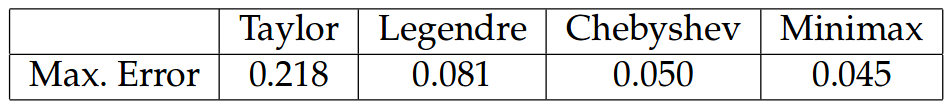
\includegraphics[scale=0.28]{ComparaisonPoly.png}
      \caption{Erreur absolue de differents polynômes apparoximant $e^x$ sur [-1,1]}
      \label{Erreur absolue de differents polynômes apparoximant $e^x$ sur [-1,1]}
    \end{center}
\end{figure}



\subsubsection{Erreur informatique}

Lors de l'execution des algorithmes, une erreur informatique s'ajoute à l'erreur mathématique due au caractère
discret et fini des nombres flottants en machine. En effet, de manière générale l'addition, la soustraction, la mutlipication
et la division entre deux nombres machines ne donne pas un nombre machine. \\
Cela se traduit par de multiples appels à la fonction d'arrondi (Round to Nearest) qui introduit une erreur
de $|\delta| < 2^{-p}$ à chaque fois comme expliqué en \hyperref[sec:arrondis]{partie 2.2}. \\ \\
Dans notre cas nous utilisons l'instruction FMA (disponible sur la plupart des processeurs récents) qui permet
de réduire de moitié le nombre d'opérations et donc d'erreurs introduites par RN appelées \textbf{erreurs d'arrondi}.
\\
Il existe aussi les \textbf{erreurs d'annulation} et les \textbf{erreurs d'absorption}, mais vu la conception
de nos algorithmes, celles-ci n'interviennent pas dans notre calcul d'erreur.

\subsection{Précision de l'algorithme arctangente/arcsinus}
\subsubsection{Erreur mathématique}

Dans le cas de l'arctangente, nous ulisons ici aussi un polynôme minimax avec des coefficients machine trouvés grâce à l'outil Sollya.
Ainsi de la même façon que pour le cosinus et le sinus, l'erreur mathématique maximale commise est donc l'erreur maximale du polynôme minimax.

\\
Une seconde source d'erreur lors de l'évaluation de arsinus est que nous sommes amenés à utiliser notre fonction square root, qui est implémenté
suivant la "Babylonian Method" ou "Méthode de Héron" qui s'appuie sur le fait que avec une valeur initiale S, la suite récurrente:

\begin{center}
\begin{equation}
  x_{n+1} = 0.5(x_{n} + S/x_{n})
\end{equation}
\end{center}

\\
\noindent converge vers racine de x. \\
La vitesse de convergence de cet algorithme depend de la valeur initiale (seed). Plus celle-ci est une estimation précise de
la valeur que l'on veut calculer, plus l'algorithme convergera rapidement.
\subsubsection{Erreur informatique}

Nous utilisons ici aussi l'instruction FMA qui n'introduit qu'une erreur machine contre deux pour une addition et une multiplication.
Il n'y a pas d'erreur dû à la range reduction depuis que l'intervalle est séparé en deux parties: [-1, 1] et le reste.
\\
\\
Il y a cependant une erreur lorsque nous utilisons la formule de réduction d'intervalle. En effet nous sommes amenés à utiliser arctangente(1/x) pour
revenir au résultat. Le fait de prendre l'inverse de l'argument entraine une erreur supplémentaire. En effet même si x est un flottant machine, il y
a très peu de chance que son inverse le soit aussi, d'où l'erreur introduite. \\
Il est également possible de trouver une valeur nulle pour un très grand x, alors que son inverse n'est pas zéro !!
Ceci étant notre fonction arctangente reste la plus précise et la plus stable de toutes nots fonctions.

\section{Tests et validations des algortihmes}
\subsection{Validation de l'implémentation en Java}
\label{sec:tests1}
\\
Afin de tester l'implémentation des nos fonctions et leur précision, nous avons établi une base de tests
graphiques pour chacune d'entre-elles. Nous prendrons la fonction cosinus comme exemple, mais les graphiques
pour les autres fonctions se trouvent en \hyperref[sec:annexes]{Annexes}.\\
\\
\\
1ère validation : confirmation visuelle de la forme :\\

\begin{figure}[ht]
    \begin{center}
      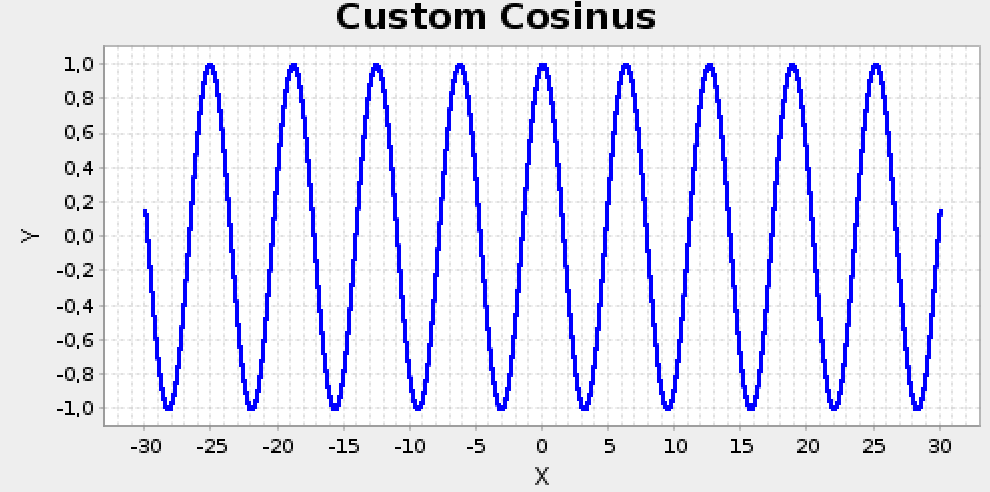
\includegraphics[scale=0.35]{CosTay.png}
      \caption{Custom cosinus sur [-30,30] avec 100 000 points}
      \label{Custom cosinus sur [-30,30] avec 100 000 points}
    \end{center}
\end{figure}

\newline
\newline
\\
\\
Une fois que cette étape est validée, nous passons à l'étude de l'erreur. \\
On prend comme référence
la classe Math.lang.java dans un premier temps. \\ \\
\newpage
2ème validation graphique : l'erreur absolue \\

\begin{figure}[ht]
    \begin{center}
      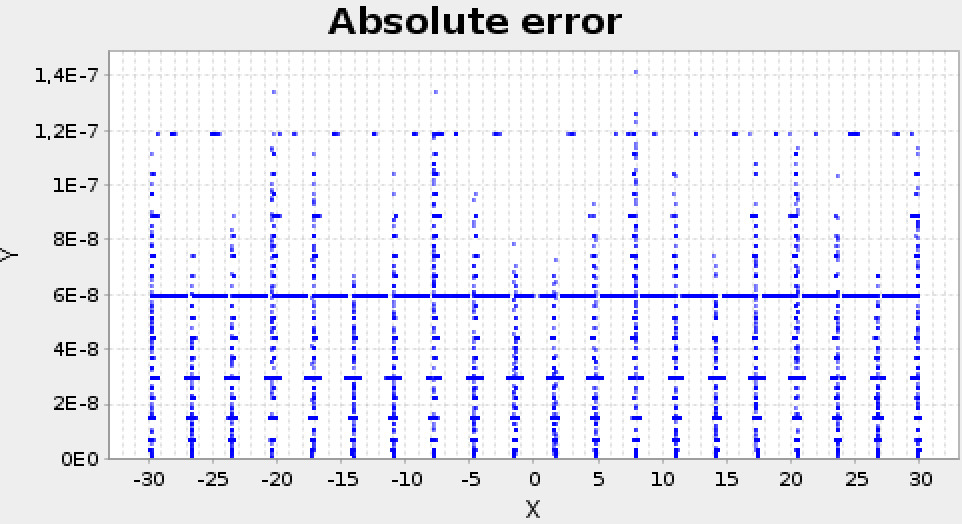
\includegraphics[scale=0.28]{ErrorAbsCosTay.png}
      \caption{Erreur absolue du cos par Maclaurin sur [-30, 30]}
      \label{Erreur absolue du cos par Maclaurin sur [-30, 30] avec 100 000 points}
    \end{center}
\end{figure}

\noindent Nous observons que celle-ci ne dépasse pas 1.4E-7. Les irrégularités que l'on peut remarquer aux abscisses
$k\pi+\frac{\pi}{2}$ (k entier relatif) seront discutées plus tard. \\ \\Avec les polynômes minimax :

\begin{figure}[ht]
    \begin{center}
      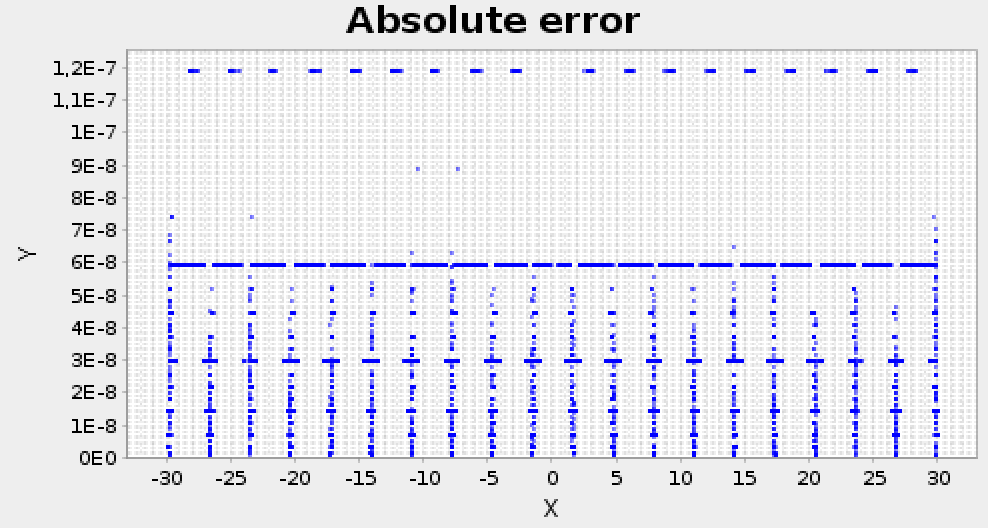
\includegraphics[scale=0.28]{ErrorAbsCosMini.png}
      \caption{Erreur absolue du cos par Polynôme Minimax sur [-30, 30]}
      \label{Erreur absolue du cos par Polynôme Minimax sur [-30, 30] avec 100 000 points}
    \end{center}
\end{figure}

Comme suggéré en \hyperref[sec:minimax]{partie 4.1.3}, nous remarquons que l'algorithme utilisant les polynômes Minimax est plus précis.\\
Il est aussi intéressant de regarder les erreurs absolues pour de grands arguments : \\ \\ \\ \\

\begin{figure}[ht]
    \begin{center}
      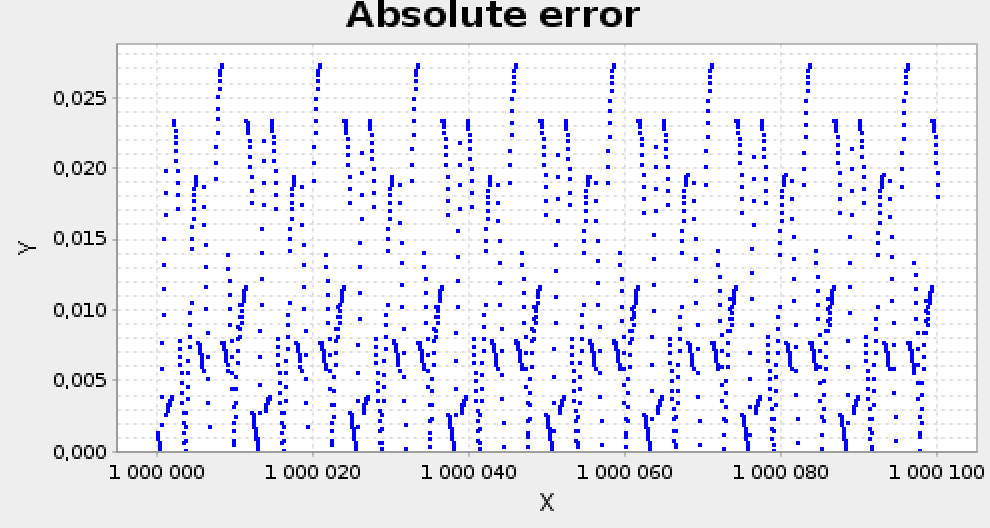
\includegraphics[scale=0.32]{ErrorAbsCosMiniFar.png}
      \caption{Erreur absolue du cos par Maclaurin sur [10^6, 10^6 + 100]}
      \label{Erreur absolue du cos par série Maclaurin sur $[10^6, 10^6 + 100]$}
    \end{center}
\end{figure}

Enfin, grâce à la fonction ULP, nous pouvons par un simple calcul déterminer à combien d'ULP
notre valeur se trouve de la valeur de java.lang.Math. C'est-à-dire combien il y a de flottants
représentables en machine entre les deux valeurs.\\
\\
\newpage
Avec series de Maclaurin :
\begin{figure}[ht]
    \begin{center}
      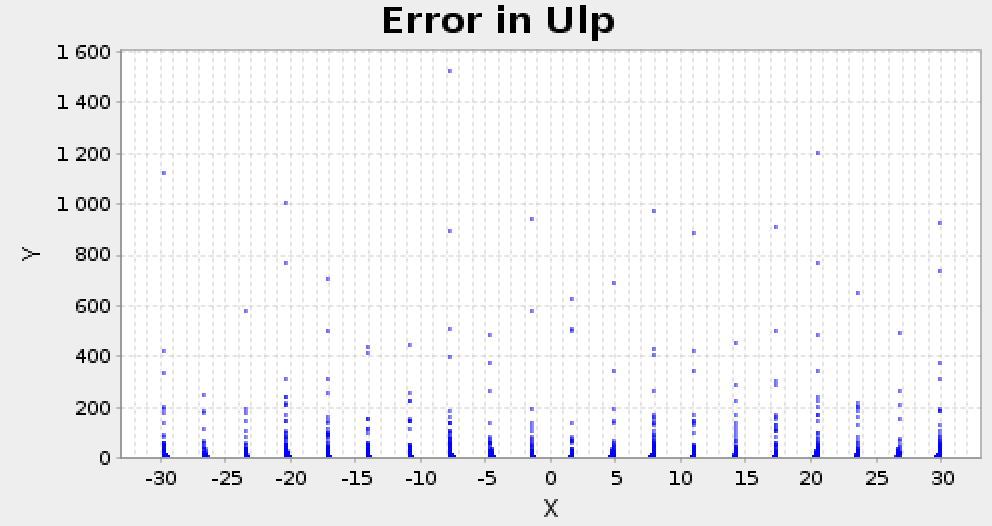
\includegraphics[scale=0.29]{ErrorUlpTay.png}
      \caption{Erreur en ulp du cos par Polynôme Minimax sur [-30, 30]}
      \label{Erreur en ulp du cos par série Maclaurin sur [-30, 30] avec 100 000 points}
    \end{center}
\end{figure}

\\ \\
Avec polynôme Minimax :

\begin{figure}[ht]
    \begin{center}
      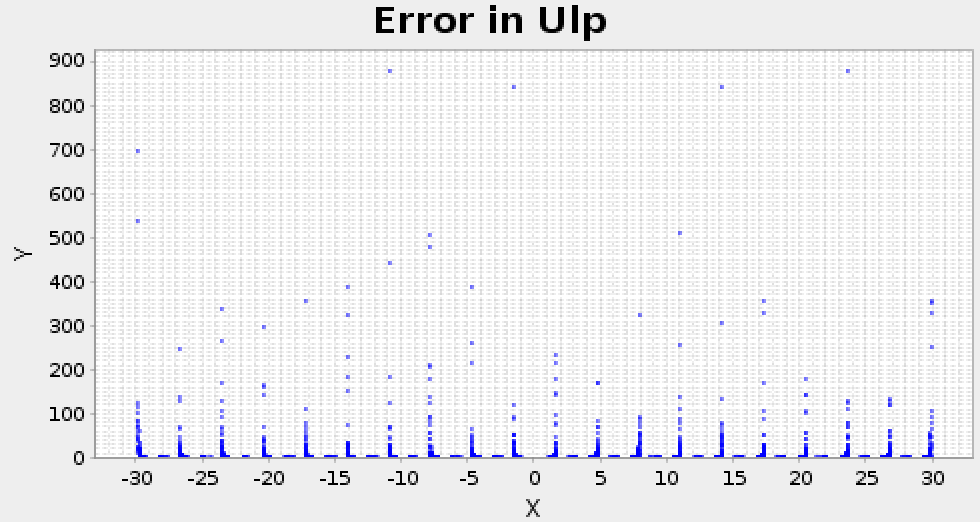
\includegraphics[scale=0.29]{ErrorUlpMini.png}
      \caption{Erreur en ulp du cos par Polynôme Minimax sur [-30, 30]}
      \label{Erreur en ulp du cos par Polynôme Minimax sur [-30, 30] avec 100 000 points}
    \end{center}
\end{figure}

Une fois encore, nous pouvons confirmer que le polynôme Minimax est plus précis.
Nottons l'importance de la validation graphique dans le cas de l'extension math. En effet pour 100 000 points en tre [-30, 30] nous obtenons \textbf{94,4\% de valeur à 0 et 1 ULP}
(testé algorithmiquement) de la valeur de Java. Ainsi en testant la classe math seulement avec le terminal en affichant seulement quelques valeurs, il y a de grandes chances de seulement tomber sur
des valeurs exactes. Nous aurions alors validé, à tort, un algorithme avec un fausse idée de sa précision.


Nous avons remarqué un phénomène récurrent concernant la précision en ULP de nos fonctions Sinus et Cosinus. Par exemple, pour le cosinus,
bien que nous ayons une erreur absolue plus ou moins constante d'une valeur de 6E-8, nous observons un gros pic de l'erreur en terme d'ULP au niveau des
abscisses $\frac{\pi}{2} + k\pi$.\\
\begin{figure}[ht]
  \begin{center}
    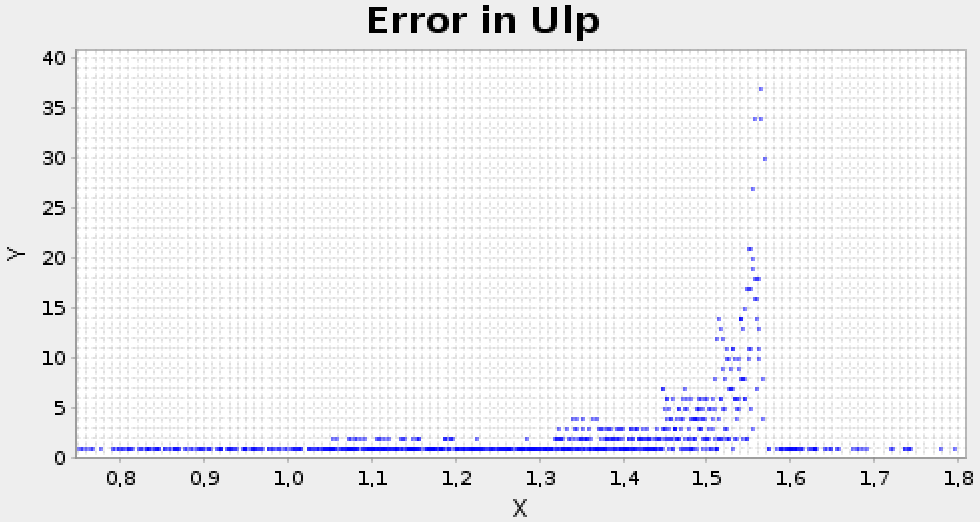
\includegraphics[scale=0.28]{PicErrorUlp.png}
    \caption{Pic d'erreur}
    \label{Erreur en ulp du cos par Polynôme Minimax sur [-30, 30] avec 100 000 points}
  \end{center}
\end{figure}
\\
Nous étions dans un premier temps déconcerté par cela, mais nous avons réalisé dans un second temps que cela était "normal". En effet, ce phénomène se produit là où les fonctions
ont une valeur très proche de 0. Or pour savoir à combien d'ULP nous sommes de la valeur Java nous faisons:

\begin{center}
\begin{equation}
  \frac{|notreValeur - javaValeur|}{ulp(javaValeur)}
\end{equation}
\end{center}

\\
\noindent Or ulp(javaValeur) est vraiment petit lorsque "javaValeur" est petit (cela est dû à la grande densité des flottants machine vers 0 voir partie \hyperref[sec:notions]{partie 2.1}).
Il est alors normal qu'une toute petite erreur en valeur absolue se traduise par des milliers d'ULP de différence.



\subsection{Un autre point de repère: Math de Python}

Comme il nous a été conseillé lors des séances de suivi de prendre un second point de comparaison pour évaluer notre classe Math (autre que celle de Java).

\begin{figure}[h!]
  \begin{center}
    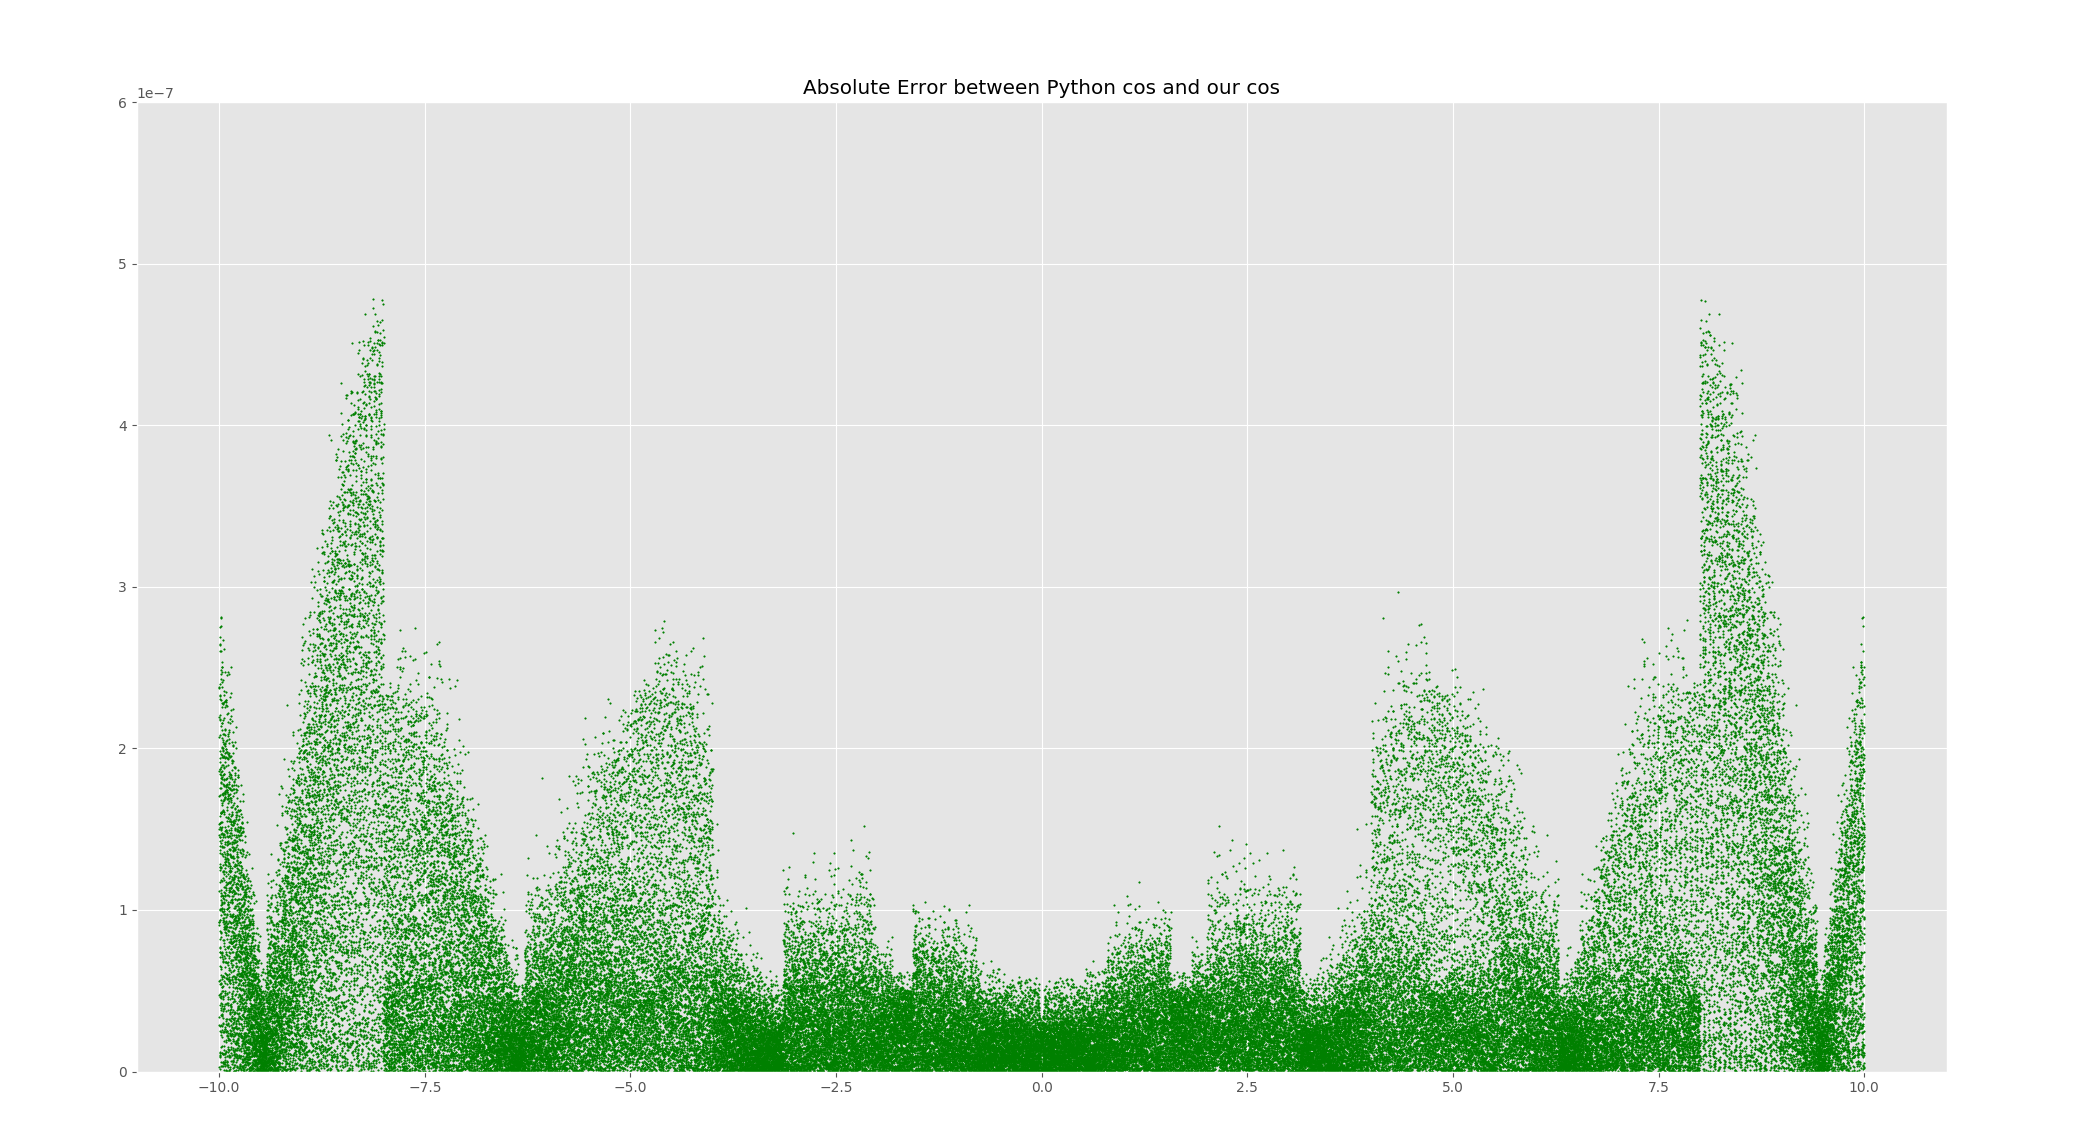
\includegraphics[scale=0.2]{ErrorAbsCosPython.png}
    \caption{Comparaison avec le Cosinus de Python}
    \label{Comparaison avec le Cosinus de Python}
  \end{center}
\end{figure}

Nous avons alors décidé de comparer nos résultats avec ceux de la classe math de Python. Nous avons réaliser cela en écrivant nos résultats dans un fichier .txt, puis
en chargant ce fichier dans python pour ensuite travailler dessu. L'affichage graphique de python utilisé est matplotlib.pyplot. Voici pour le Cosinus, l'erreur absolue que
nous obtenons. Nous remarquons alors que les erreurs absolues avec la librarie de python sont sensiblement les mêmes que celles obtenues avec Java (erreur en $10^{-7}$).


\subsection{Validation de l'implémentation en Deca}

Les difficultés de l'implémentation en Déca ont été sous-estimé par notre groupe. Tout d'abord, la class Math utilisant l'instruction
FMA des processeurs (Math.fma() en Java), nous devions dans un premier temps gérer la méthode ASM du compilateur Decac, afin de nous
permettre d'introduire une méthode en assembleur dans notre classe Math.\\
\\
Ceci étant fait, nous nous sommes rendu compte que malgré nos 250 scripts de tests, il restait beaucoup, beaucoup d'erreur dans des cas
auxquels nous n'avions pas pensé. La plupart de ces erreurs viennent de la génération de code assembleur dans la partie C et ont été
révélés par le code de la classe Math.\\
\\
Ceci étant, nous ne sommes pas parvenu à une implémentation totale de la classe Math (qui est tout à fait opérationnelle en Java) en Déca.
Ainsi il n'était pas possible pour moi de réaliser des tests sur la classe Math en Déca.
Tout le code compile, mais il y a certaines fonctions essentielles qui provoquent des erreurs à l'exécution.\\
Nottons tout de même que le code de Math.deca devrait très bien fonctionner sur un compilateur plus abouti que le notre.

\begin{thebibliography}{5}

\bibitem{paper1}Floating Point Math Functions, de Frank.J. Testa \url{http://www.microchip.com/stellent/groups/techpub_sg/documents/appnotes/en010982.pdf}.

\bibitem{paper2}COMPUTING ACCURATE HORNER FORM APPROXIMATIONS, d'un étudiant NSERC Doctoral Scholarship \url{https://arxiv.org/pdf/1508.03211.pdf}.

\bibitem{sollya}Sollya Tools \url{http://sollya.gforge.inria.fr/}.

\bibitem{elementaryFunctions}Elementary Functions, Jean-Michel M \url{https://doc.lagout.org/science/0_Computer%20Science/2_Algorithms/Elementary%20Functions_%20Algorithms%20and%20Implementation%20%282nd%20ed.%29%20%5BMuller%202005-10-24%5D.pdf}.
\end{thebibliography}
\\

\newpage
\section{Annexes}
\label{sec:annexes}

\subsection{Graphiques du Cosinus}

\begin{figure}[h!]
  \begin{center}
    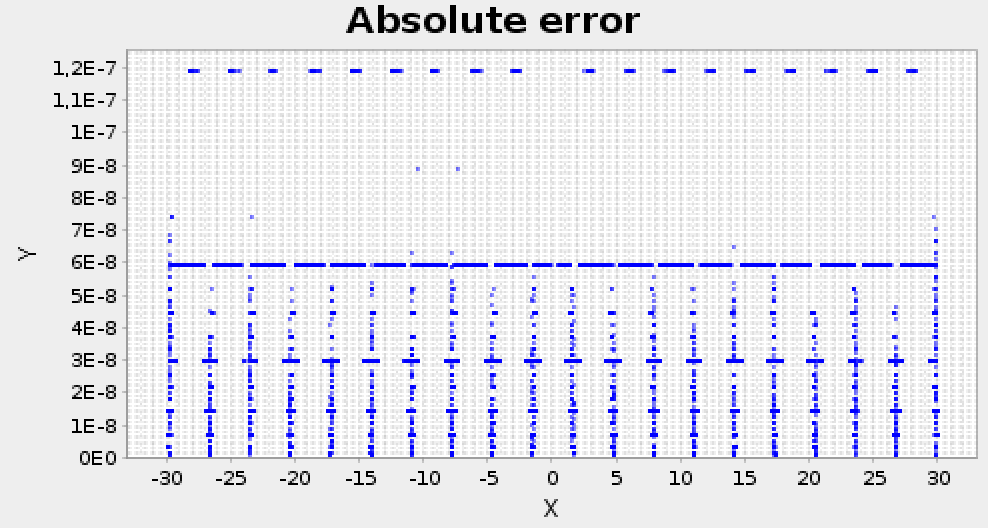
\includegraphics[scale=0.33]{ErrorAbsCosMini.png}
    \caption{Erreur absolue du Cosinus avec 100 000 points sur [-30,30]}
    \label{Erreur asolue du Cosinus avec 100 000 points sur [-30,30]}
  \end{center}
\end{figure}
\begin{figure}[h!]
  \begin{center}
    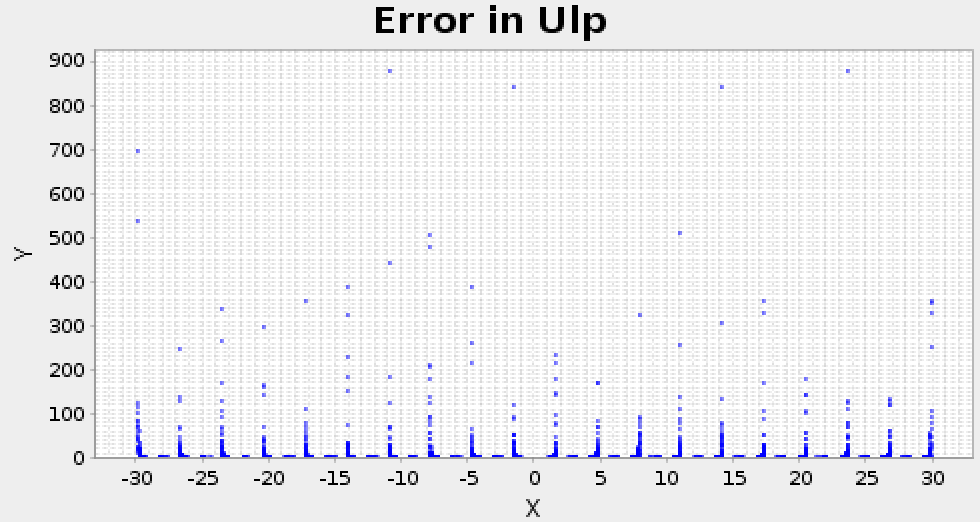
\includegraphics[scale=0.33]{ErrorUlpMini.png}
    \caption{Erreur en ULP du Cosinus avec 100 000 points sur $[-30,30]$}
    \label{Erreur en ULP du Cosinus avec 100 000 points sur $[-30,30]$}
  \end{center}
\end{figure}
\begin{figure}[h!]
  \begin{center}
    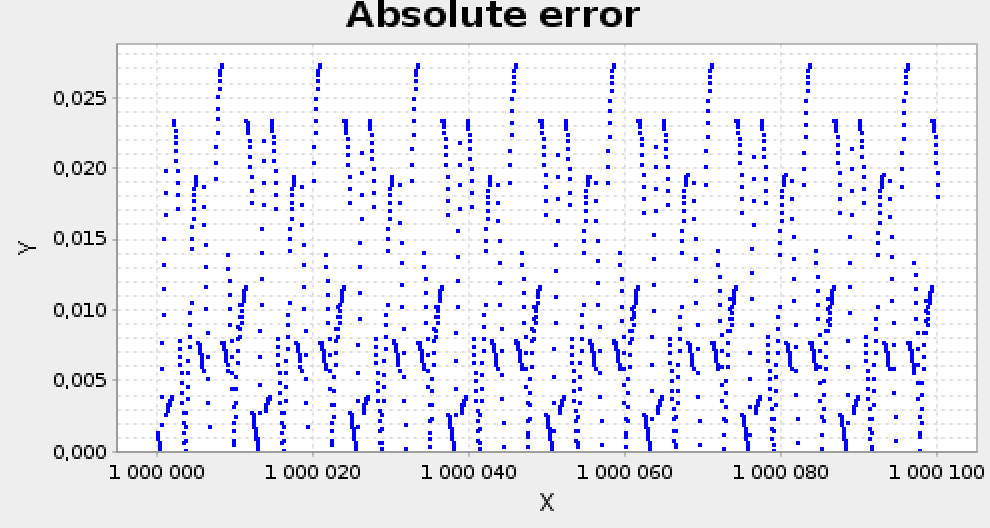
\includegraphics[scale=0.33]{ErrorAbsCosMiniFar.png}
    \caption{Erreur absolue du Cosinus avec 100 000 points sur $[10^6,10^6+100]$}
    \label{Erreur absolue du Cosinus avec 100 000 points sur $[10^6,10^6+100]$}
  \end{center}
\end{figure}

\newpage
\subsection{Graphiques du Sinus}

\begin{figure}[h!]
  \begin{center}
    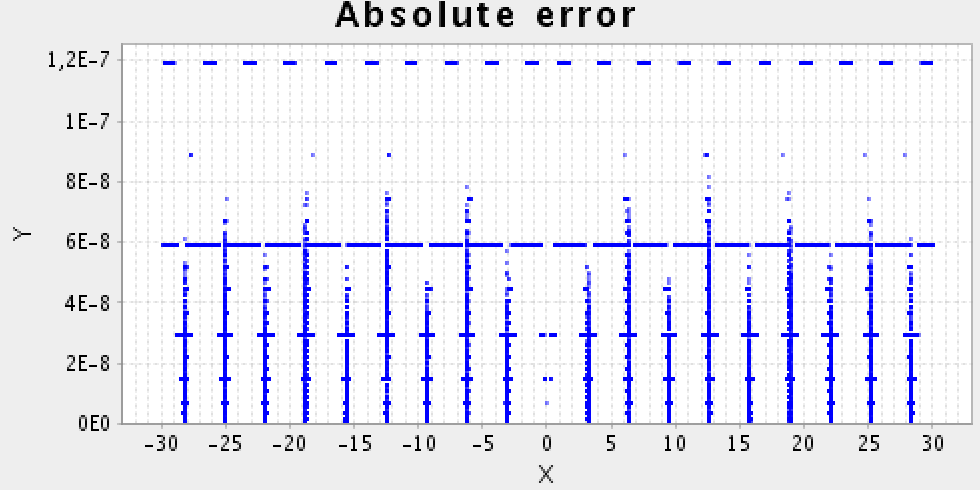
\includegraphics[scale=0.33]{sinus_abs.png}
    \caption{Erreur absolue du Sinus avec 100 000 points sur [-30,30]}
    \label{Erreur absolue du Sinus avec 100 000 points sur [-30,30]}
  \end{center}
\end{figure}

\newpage

\begin{figure}[h!]
  \begin{center}
    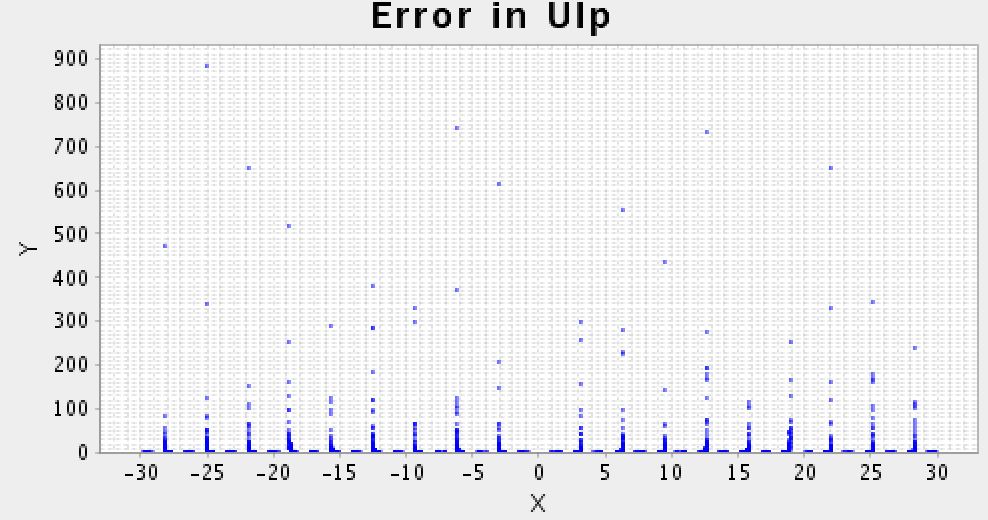
\includegraphics[scale=0.33]{sinus_ulp.png}
    \caption{Erreur en ULP du Sinus avec 100 000 points sur $[-30,30]$}
    \label{Erreur en ULP du Sinus avec 100 000 points sur $[-30,30]$}
  \end{center}
\end{figure}
\begin{figure}[h!]
  \begin{center}
    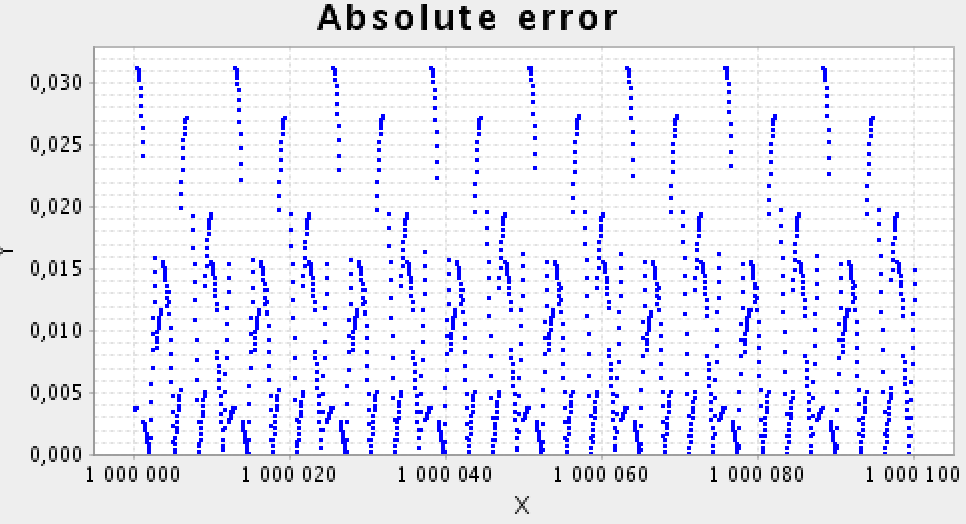
\includegraphics[scale=0.33]{sinus_far.png}
    \caption{Erreur absolue du Sinus avec 100 000 points sur $[10^6,10^6+100]$}
    \label{Erreur absolue du Sinus avec 100 000 points sur $[10^6,10^6+100]$}
  \end{center}
\end{figure}

\newpage

\subsection{Graphiques de l'ULP}

\begin{figure}[h!]
  \begin{center}
    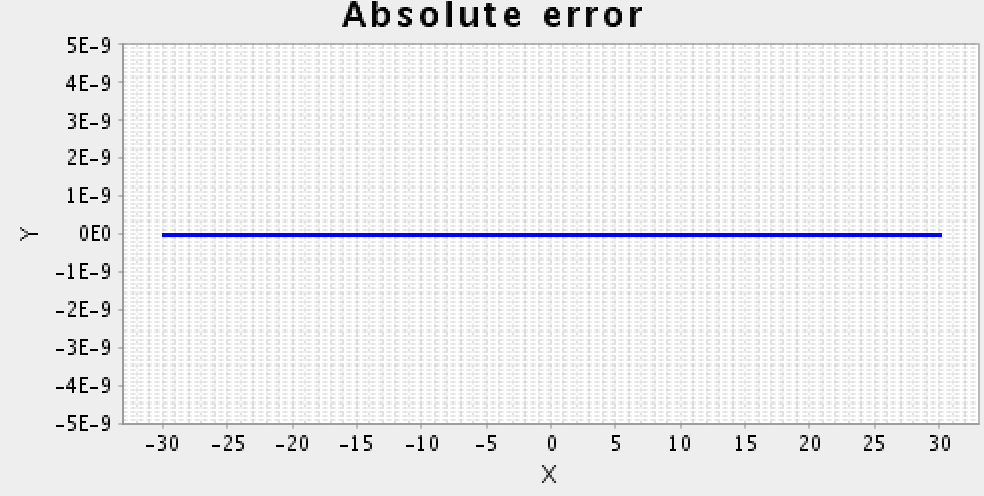
\includegraphics[scale=0.33]{ulp_abs.png}
    \caption{Erreur absolue de ULP avec 100 000 points sur [-30,30]}
    \label{Erreur absolue de ULP avec 100 000 points sur [-30,30]}
  \end{center}
\end{figure}
\begin{figure}[h!]
  \begin{center}
    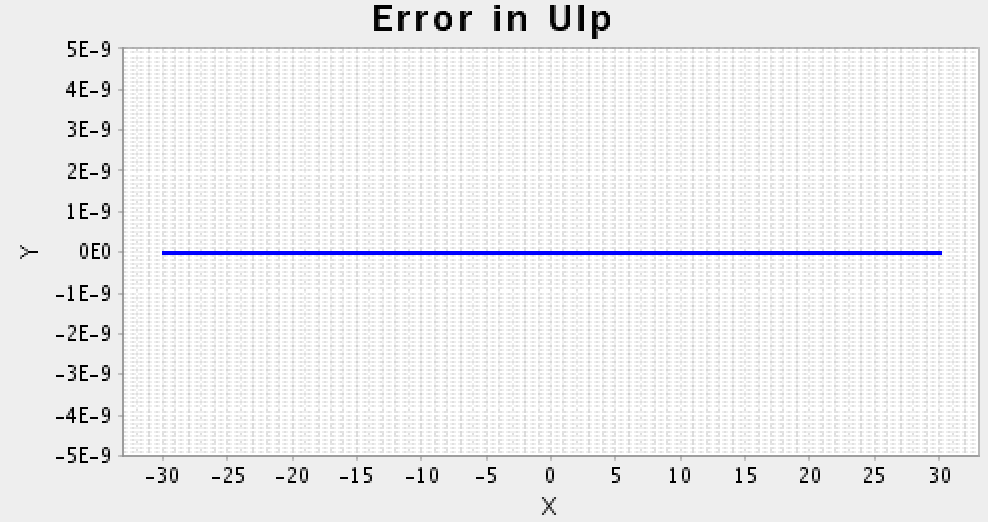
\includegraphics[scale=0.33]{ulp_ulp.png}
    \caption{Erreur en ULP de ULP avec 100 000 points sur $[-30,30]$}
    \label{Erreur en ULP de ULP avec 100 000 points sur $[-30,30]$}
  \end{center}
\end{figure}
\newpage

\begin{figure}[h!]
  \begin{center}
    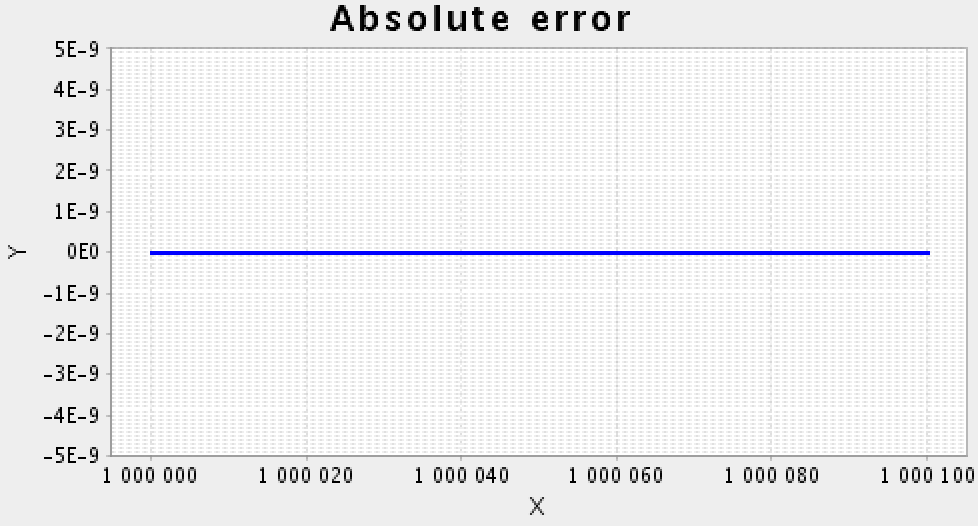
\includegraphics[scale=0.33]{ulp_far.png}
    \caption{Erreur absolue de ULP avec 100 000 points sur $[10^6,10^6+100]$}
    \label{Erreur absolue de ULP avec 100 000 points sur $[10^6,10^6+100]$}
  \end{center}
\end{figure}
\subsection{Graphiques du Arctangente}

\begin{figure}[h!]
  \begin{center}
    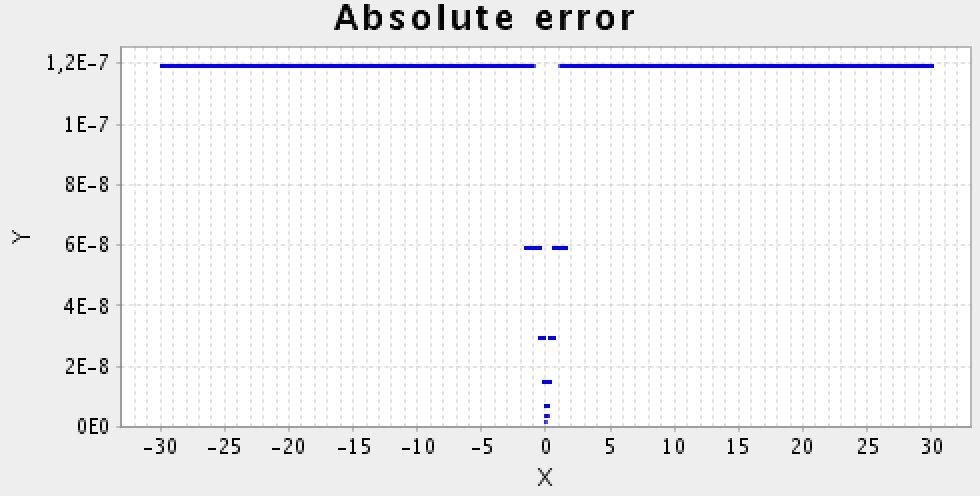
\includegraphics[scale=0.33]{atan_abs.png}
    \caption{Erreur absolue de arctangente avec 100 000 points sur [-30,30]}
    \label{Erreur absolue de arctangente avec 100 000 points sur [-30,30]}
  \end{center}
\end{figure}

\newpage
\begin{figure}[h!]
  \begin{center}
    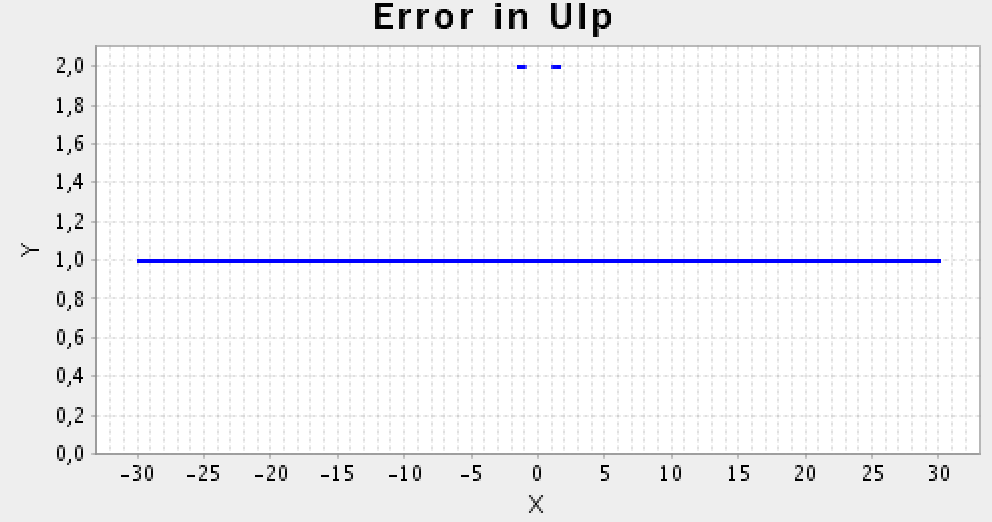
\includegraphics[scale=0.33]{atan_ulp.png}
    \caption{Erreur en ULP de arctangente avec 100 000 points sur $[-30,30]$}
    \label{Erreur en ULP de arctangente avec 100 000 points sur $[-30,30]$}
  \end{center}
\end{figure}
\begin{figure}[h!]
  \begin{center}
    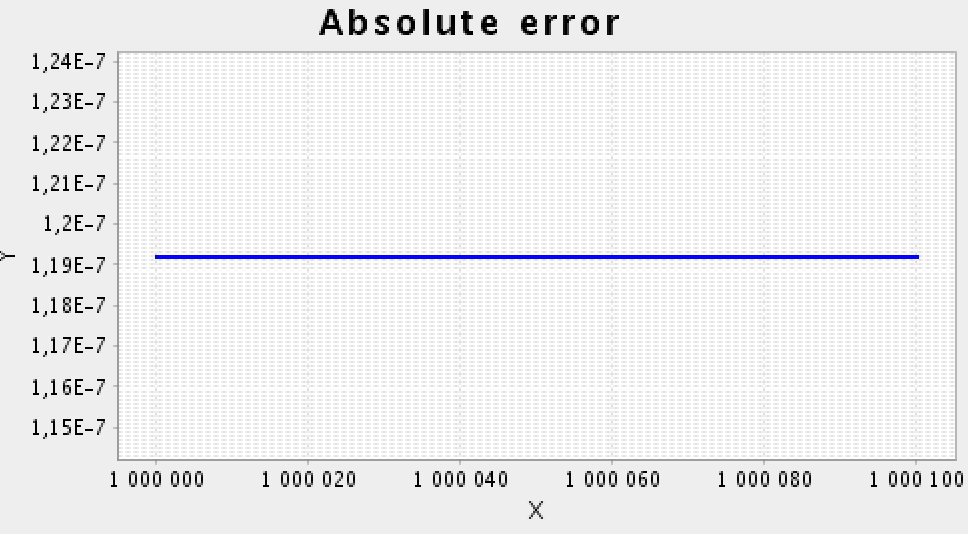
\includegraphics[scale=0.33]{atan_far.png}
    \caption{Erreur absolue de arctangente avec 100 000 points sur $[10^6,10^6+100]$}
    \label{Erreur absolue de arctangente avec 100 000 points sur $[10^6,10^6+100]$}
  \end{center}
\end{figure}
\newpage
\subsection{Graphiques du Arcsinus}
\begin{figure}[h!]
  \begin{center}
    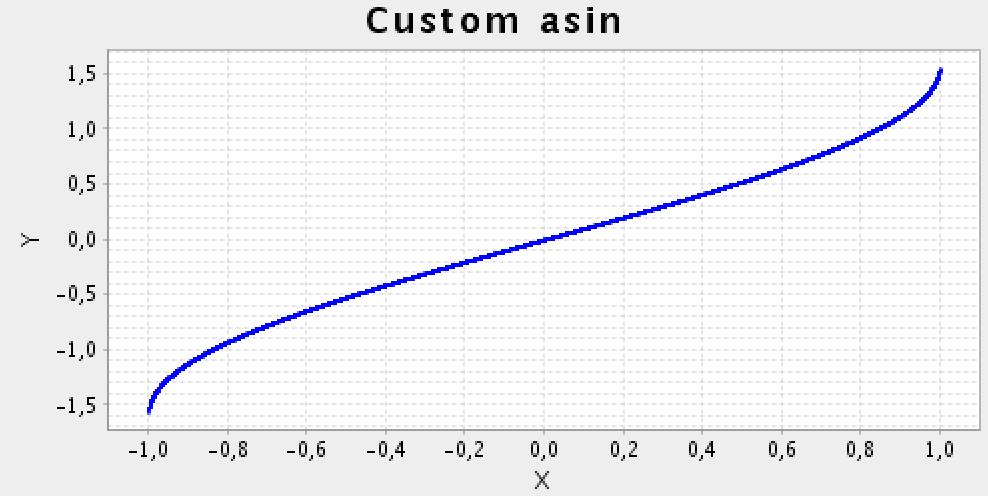
\includegraphics[scale=0.33]{asin.png}
    \caption{Fonction arcsinus avec 100 000 points}
    \label{Fonction arcsinus avec 100 000 points}
  \end{center}
\end{figure}
\begin{figure}[h!]
  \begin{center}
    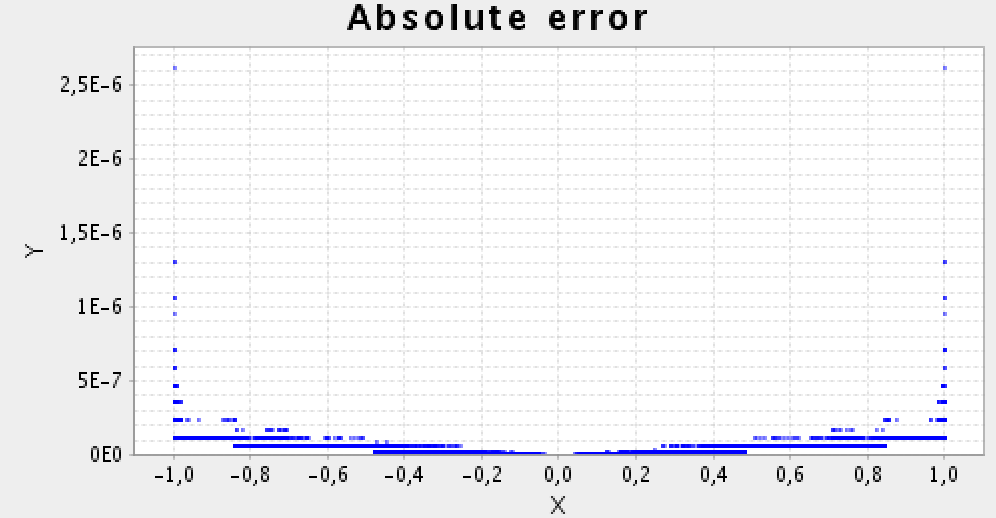
\includegraphics[scale=0.33]{asin_abs.png}
    \caption{Erreur absolue de arcinus avec 100 000 points}
    \label{Erreur absolue de arcinus avec 100 000 points}
  \end{center}
\end{figure}
\begin{figure}[h!]
  \begin{center}
    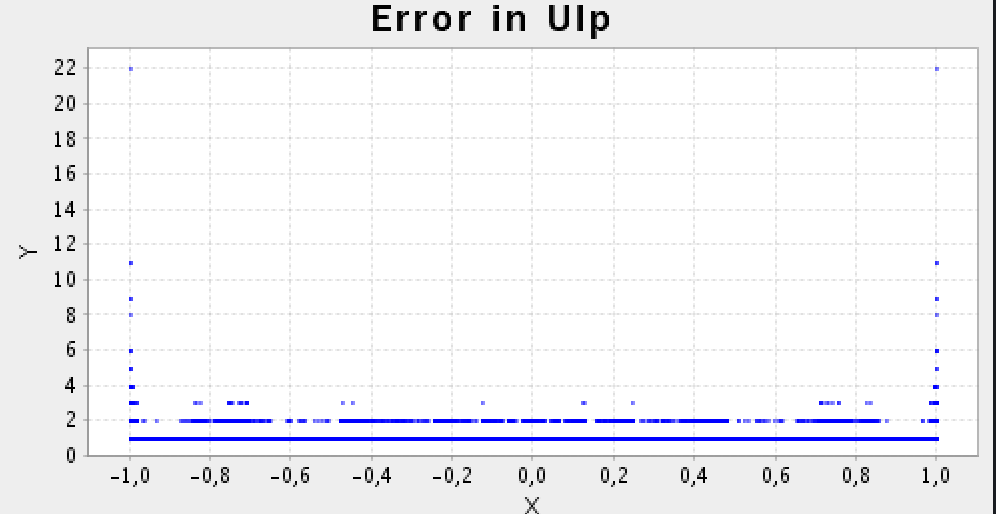
\includegraphics[scale=0.33]{asin_ulp.png}
    \caption{Erreur en ULP de arcsinus avec 100 000 points}
    \label{Erreur en ULP de arcsinus avec 100 000 points}
  \end{center}
\end{figure}
\end{document}
